\documentclass[../notes.tex]{subfiles}
\graphicspath{
    {"../figures"}
}

\begin{document}

\subsection{Finishing Last Lecture}
From the previous lecture:

\[
				\dv{t} x + \frac{3x}{60+2t} = \frac{1}{2}
.\]

How much salt is in the tank when it is full? First, find out how full the tank is (given that it holds 100 Litres):

\begin{equation*}
				60 + 2t = 100 \implies t=20 \text{ minutes}
\end{equation*}

Now use the integration factor $r(t)=e^{\int p(x) \dd x}$.

\begin{align*}
				r(t) &= e^{\int \frac{3}{60+2t} \dd t} & \\
				(u = 60 + 2t &\implies \dd u = 2 \dd t) \\
				r(t) &= e^{ \frac{3}{2} \int \frac{1}{u} \dd u} = e^{\frac{3}{2} \ln{60 + 2t}} \\
				r(t) &= (60+2t)^{\frac{3}{2}}
\end{align*}

Now utilize inverse product rule:

\begin{align*}
				\dv{t} (60+2t)^{\frac{2}{3}} + \frac{3x}{60+2t} (60+2t)^{\frac{2}{3}} &= \frac{1}{2} (60+2t)^{\frac{2}{3}} \\
				\int \dv{t} \left[ x(t) (60+2t) \right] ^{\frac{2}{3}} &= \int \frac{1}{2} (60+2t)^{\frac{2}{3}} \\
				(60+2t)^{\frac{2}{3}} = \frac{1}{2} \cdot \frac{1}{2} \cdot \frac{2}{5} (60+2t)^{\frac{5}{2}} + c &= \frac{1}{10} (60+2t)^{\frac{5}{2}} + c \\
				x(t) &= \frac{1}{10} (60+2t) + C(60+2t)^{\frac{-3}{2}}
.\end{align*}

Then applying the initial condition:

\[
				x(0) = \frac{1}{10} (60) + C(60)^{-\frac{3}{2}} \implies \boxed{C \approx 1860.}\]

Now plug in $t=20$

\[
				x(20) = \frac{1}{10}(60+40) + 1860(60 + 40)^{-\frac{3}{2}} \approx \boxed{11.86 \text{kg}.}\]

\subsubsection{Solving Tank Problems}
\label{sec:tankproblems}

Consider a tank of brine water or some dissolved substance in a solvent. Commonly it is brine water. The tank has both an input and output. The input liquid comes in at a rate $r_1$ with a concentration of $c_1$. The output is almost always considered to be homogeneous since it is at the bottom of the tank. The output rate is $r_2$ and output concentration is $c_2$. The overall quantity of solute is $s(t)$ and tank volume is  $v(t)$. The setup is represented by \ref{fig:singletank}.

\begin{figure}[htpb]
    \centering
				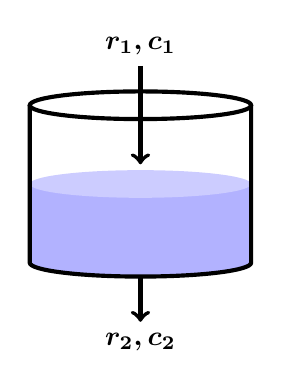
\begin{tikzpicture}[
								scale=1,
								line width=1.5pt,
								]
								\draw [->] (0,2.50) -- (0,1.25) node [pos = 0, above, font=\boldmath] (r1) {$r_1, c_1$};
								\draw (0,2) ellipse [x radius = 40pt, y radius=5pt];
								\draw [->] (0,0) -- (0,-0.75) node [below,font=\boldmath] (r2) {$r_2, c_2$};
								\fill[blue!30] (-40pt,1) -- (-40pt, 0) arc [start angle=180, end angle=360, x radius = 40pt, y radius=5pt] -- (40pt, 0) -- (40pt, 1);
								\fill[blue!20] (0, 1) ellipse [x radius = 40pt, y radius=5pt];
								\draw (-40pt,2) -- (-40pt, 0) arc [start angle=180, end angle=360, x radius = 40pt, y radius=5pt] -- (40pt, 0) -- (40pt, 2);
				\end{tikzpicture}
				\caption{Singular Tank System}
				\label{fig:singletank}
\end{figure}

From the setup, one can determine that:
\[
\Delta s = r_1 c_1 \Delta t - r_2 c_2 \Delta t
.\]

{ Dividing by $\Delta t$ and taking the limit arrives at the differential equation
\[
				\boxed{\dv{s}{t} = r_1 c_1 - r_2 c_2
.}\] }

\subsection{Substitution}

Nice types of ODES:
\begin{align*}
				& y'=f(x) & y'=f(x,y)=h( x ) \cdot g( y ) &\\
				& y'=f(y) & \dv{y}{t} + p( t ) x = f( t ) &
.\end{align*}

The last case represents a linear, first order differential equation. Via the integration factor, they are easy to solve. In certain cases, an equation may not look linear or separable; however, \textbf{change of variables} can resolve certain cases like this.

\begin{stickynote}{Substitutions}
				\textbf{General substitutions that work}:
				{\def\arraystretch{1.5}
				\setlength{\arrayrulewidth}{1pt}
				\begin{center}
								\begin{tabular}{| a | a |}\hline
												$y'=F(ax + by)$ & $v=ax+by$ \\\hline
								$y'=G(\frac{y}{x})$ & $v=\frac{y}{x}$ \\\hline
								$y'+p(x) y = q(x) y^{n}$ & $v=y^{1-n}$ \\\hline
				\end{tabular}
\end{center}}
\end{stickynote}

\begin{example}{Find the general solution of $y' = (4x - y + 1)^2$}
Let $v = 4x - y$. Rewrite in terms of v:
\begin{align*}
				& v' = 4 - y' \\
				& \downarrow \\
				& y' = 4 - v'
\end{align*}
Now:
\[
4-v' = (v + 1)^2 \implies v' = 4 - (v+1)^2
.\]
Note that it is now a separable equation.
\begin{align*}
				\frac{v'}{4-(v+1)^2} = 1 \implies -\int\frac{v'}{4-(v+1)^2} dv &= \int 1 \dd x \\
				-\frac{1}{4} \qty[\ln{\abs{ v-1 }} - \ln{\abs{ v+3 }}] &= x+c \\
				\ln{\abs{ \frac{v-1}{v+3} } } &= -4x + c \\
				\frac{v-1}{v+3} &= Ae^{-4x} \\
				v &= \frac{1+3Ae^{-4x}}{1-Ae^{-4x}}
.\end{align*}
Now that the solution is found, rewrite v back in terms of y.
\begin{align*}
				v = \frac{1+3Ae^{-4x}}{1-Ae^{-4x}} \implies 4x-y &= \frac{1+3Ae^{-4x}}{1-Ae^{-4x}} &\\
				y &= 4x - \frac{1+3Ae^{-4x}}{1-Ae^{-4x}}
.\end{align*}
\end{example}


Example where $v=\frac{y}{x}$:
\begin{example}{Solve $x^2 y' = y^2 + xy$}
\begin{align*}
\intertext{First try dividing by the highest power of the independent variable ($x^2$)}
y' &= \frac{y^2}{x^2} + \frac{y}{x} \\
\intertext{Now use $v=\frac{y}{x}$}
y' &= v^2 + v
\intertext{Find $y'$ in terms of $v$}
				v &= \underbrace{\frac{y}{x}}_{\clap{\scriptsize Quotient rule}} \\
				v' &= \frac{xy' - y}{x^2} \\
				v' &= \frac{y'}{x} - \frac{y}{x^2} \\
				v'x &= y' - \frac{y}{x} \\
				v'x &= y' - v \\
				y' &= v'x + v
\intertext{Substitute back into ODE:}
				xv' &= v^2 + v \\
				v' &= \frac{v^2}{x} \\
				\frac{v'}{v^2} &= \frac{1}{x} \\
				\int \frac{1}{v^2} \dd v &= \int \frac{1}{x} \dd x \\
				-\frac{1}{v} &= \ln( x ) + c \\
				v &= -\frac{1}{\ln( x ) + c}
\intertext{Now plug back in y for v:}
				\frac{y}{x} &= -\frac{1}{\ln( x ) + c} \\
				y &= -\frac{x}{\ln( x ) + c}
.\end{align*}
\end{example}

\subsubsection{Solving a Bernoulli Equation}


Given an equation in the form of a Bernoulli Equation, such as:

\begin{equation*}
				y' + \frac{4}{x} y = x^3y^2, x > 0
\end{equation*}

Since $n=2$, let  $v( x ) = y^{-1}$. Find $v'( x ) $

\[
				v'(x) = \dv{x} v = -y^{-2} y'
.\]


Divide the ODE by $y^{n}$:

\[
y^{-2} y' + \frac{4}{x} y^{-1} = x^3
.\]

\[
-v' + \frac{4}{x} v = x^3
.\]


Rearrange into standard linear ODE form:

\[
v' - \frac{4}{x} v = -x^3
.\]


Utilize the integration factor $\displaystyle r( x ) = e^{-\int \frac{4}{x} \dd x} = x^{-4}$

\begin{align*}
				v' - \frac{4}{x} v &= -x^3 \\
				v'r( x ) - \frac{4}{x} v r( x )  &= -x^3 r( x ) \\
				\underbrace{x^{-4}v' - x^{-4}\frac{4}{x} v}_{\clap{Inverse Product Rule}}  &= -\frac{1}{x} \\
				\dv{x} ( x^{-4} v ) &= -\frac{1}{x} \\
				x^{-4} v &= -\ln( x ) + c\\
				v &= -x^{4} \ln( x ) + cx^{4}
.\end{align*}


Plug $y$ back in for $v$:

\[
				\boxed{y(x) = \frac{1}{-x^{4}\ln( x ) + cx^{4}}.}
\]

\subsection{\nth{2} Order Linear Equations}

\begin{stickynote}{General form of \nth{2} Order Linear ODE}
				\[
				A( x ) y'' + B( x ) y' + C( x ) y = F( x )
				.\]
\end{stickynote}
\begin{theorem}{\nth{2} Order Linear ODE Solution Existence and Uniqueness}{uniqueness}
For an ODE of form $y'' + B(x) y' + C(x) y = D(x)$ with $B(x),C(x)$ and $D(x)$ as continuous functions on an interval $I$, for some  $a \in I$ and some ${b_0,b_1} \in \mathbb{R}$, a unique solution must exist and satisfy:
\[
\begin{cases}
				y'' + B(x)y' + C(x)y = D(x) \\
				y(a) = b_0 \\
				y'(a) = b_1
\end{cases}
\]
\end{theorem}
\begin{stickynote}{Homogeneous Equation}
				\[
				ay'' + by' + cy = 0 \leftarrow \text{Since this is zero, it is homogeneous}
				.\]
\end{stickynote}

\subsubsection{Superposition Principle}

Consider $y'' -k^2y = 0$.
A possible solution is $y_1 = e^{kx}$.
Therefore $y_1' = k e^{kx}$ and $y_1'' = k^2 e^{kx}$.
Plugging into the original ODE: \newline

\centerline{$\boxed{y_1'' -k^2y_1 = \left( k^2e^{kx} \right) - k^2\left( e^{kx} \right)=0 \: \checkmark }$}
$\newline$
Another solution is $y_2=e^{-kx}$. By the \namethmref{th:superposition}, their linear combination is also a solution. In this instance, for $c_1, c_2 \in \mathbb{R}$:

\begin{theorem}{Superposition Principle}{superposition}
				For any linearly homogeneous differential equation, if it has two solutions $y_1(t)$ and $y_2(t)$, then the function:
				\[
				y(t) = c_1 y_1(t) + c_2 y_2(t)
				.\]
				Is also a solution.
\end{theorem}

\subsubsection{The Wronskian}
In the case of an \nth{2} Order Linear Homogeneous equation, utilizing the \namethmref{th:superposition} offers new solutions to the ODE. However, the linear combination may not always result in a general solution. Inspect the general form the ODE:
\[
p(t)y'' + q(t)y' + r(t)y = 0 \implies
\begin{cases}
				y(t_0) &= y_0 \\
				y'(t_0) &= y_1
\end{cases}
.\]
By the \nameref{th:superposition}
\[
				y(t) = c_1 y_1(t) + c_2 y_2(t)
.\]
Both $y_1$ and $y_2$ must satisfy the initial conditions in order to provide a general solution. Find the value of the constants $c_1$ and $c_2$.
\begin{align*}
				y_0 &= y(t_0) = c_1 y_1(t_0) + c_2 y_2(t_0) \\
				y_1 &= y'(t_0) = c_1 y_1'(t_0) + c_2 y_2'(t_0)
.\end{align*}

Rewrite in terms of a system of matrices
{
\newcommand{\A}{\mqty|
								y_1(t_0) & y_2(t_0) \\
								y_1'(t_0) & y_2'(t_0)
				|}
\[
\underbrace{\A}_{\vb{A}}
\underbrace{\mqty[c_1 \\ c_2]}_{\vb{x}} = \underbrace{\mqty[y_0 \\ y_1]}_{\vb{b}}
\]
Note that $c_1$ and $c_2$ can be solved using Cramer's Rule
\begin{align*}
				&
				c_1 = \frac{\mqty|
								y_0 & y_2(t_0) \\
								y_1 & y_2'(t_0)
				|}{\A}. &
				c_2 = \frac{\mqty|
								y_1(t_0)& y_0 \\
								y_1'(t_0)& y_1
				|}{\A}.
				&
\end{align*}}

This restatement of the imposed initial value conditions reveals a new, succinct condition to check for generality. If the denominator of either $c_1$ or $c_2$ is 0, the linear combination of $y_1$ and $y_2$ will not be the general solution of the ODE. This denominator is called \namethmref{th:wronskian}.

\begin{theorem}{The Wronskian}{wronskian}
				\[
								W(f,g)(t) = \mqty|
												f(t) & g(t) \\
												f'(t) & g'(t) |
				.\]

				For a \nth{2} Order Linear Homogeneous equation, if $W(y_1,y_2)(t)\neq0$, then $y(x) = c_1 y_1 + c_2 y_2$ is a general solution to the ODE.
\end{theorem}

\begin{stickynote}{Extension of the Wronskian}
				For any $n^{\text{th}}$ order ODE, the Wronskian can be generalized. Generalizing by example, consider a \nth{3} order linearly homogeneous ODE.
				\[
				a(t)y''' + b(t)y'' + c(t)y' + d(t)y = 0
				.\]
By the \namethmref{th:superposition}, the solution is
\[
y(t) = c_1 y_1(t) + c_2 y_2(t) + c_3 y_3(t)
.\]

Like in \thmref{th:wronskian}
\begin{align*}
				y_0 &= c_1 y_1(t_0) + c_2 y_2(t_0) + c_3 y_3(t_0) \\
				y_1  &= c_1 y_1'(t_0) + c_2 y_2'(t_0) + c_3 y_3'(t_0) \\
				y_2  &= c_1 y_1''(t_0) + c_2 y_2''(t_0) + c_3 y_3''(t_0)
\end{align*}

Which as prior can be written as a matrix multiplication. This holds for any order, therefore we can right the Wronskian generally as:

\[
W(y_1,y_2,\ldots,y_n)(t) =
\mqty|
y_1(t) & y_2(t) & \ldots & y_n (t) \\
y_1'(t) & y_2'(t) & \ldots & y_n'(t) \\
\vdots & \vdots & \ddots & \vdots \\
y_1^{n}(t) & y_2^{n}(t) & \ldots & y_n^{n}(t) \\
|
\]

\end{stickynote}

\end{document}
